\documentclass[11pt, a4paper]{article}

\usepackage[czech]{babel}
\usepackage[utf8]{inputenc}
\usepackage[T1]{fontenc}
\usepackage[unicode]{hyperref}
\usepackage[left=2cm, top=3cm, text={17cm, 24cm}]{geometry}
\usepackage{times}
\usepackage{graphicx}
\usepackage{pdflscape}

\begin{document}
	\begin{titlepage}
		\begin{center}
			
\includegraphics[width=0.77 \linewidth]{FIT_logo.pdf} \\

			\vspace{\stretch{0.382}}

			\Huge{Projekt 1.~část} \\
			\Huge{Datový model (ERD), model případů užití} \\
			\LARGE{\textbf{Zoologická záhrada}} \\
			\Large{Databázové systémy}

			\vspace{\stretch{0.618}}
		\end{center}

		{\Large
			\today
			\hfill
			\begin{tabular}{ll}
			Samuel Dobroň & \href{mailto:xdobro23@stud.fit.vutbr.cz}{\texttt{xdobro23@stud.fit.vutbr.cz}} \\
            Juraj Remeň & \href{mailto:xremen02@stud.fit.vutbr.cz}{\texttt{xremen02@stud.fit.vutbr.cz}}
\end{tabular}
}
	\end{titlepage}
		\tableofcontents
		\section{Zadanie}
		Navrhněte informační systém pro zoologickou zahradu. V zoologické zahradě jsou živočichové umístěni do klecí, výběhů, či do klecí v pavilonech. Živočichové jsou děleni podle třídy, řádu, čeledě, rodu a druhu (např. lama alpaka je v třídě savců, řádu sudokopytníků, v čeledi velbloudovitých, v rodu lama a druhu alpaka). Pro zjednodušení předpokládejte striktně hierarchické dělení živočichů a to, že každý živočich je příslušníkem právě jednoho druhu. Jeden druh živočicha může být v několika výbězích či klecích, a naopak, v jednom výběhu či kleci může být více různých druhů. Systém musí být schopný vyhledávat živočichy podle jejich příslušností do jednotlivých kategorií. Pro každého živočicha je třeba uchovávat informace o datu narození (a případně úmrtí), jméno, historii výsledků měření (hmotnosti, rozměrů, ...), apod.
		\section{Use Case Diagram}
		\scalebox{0.8}{
		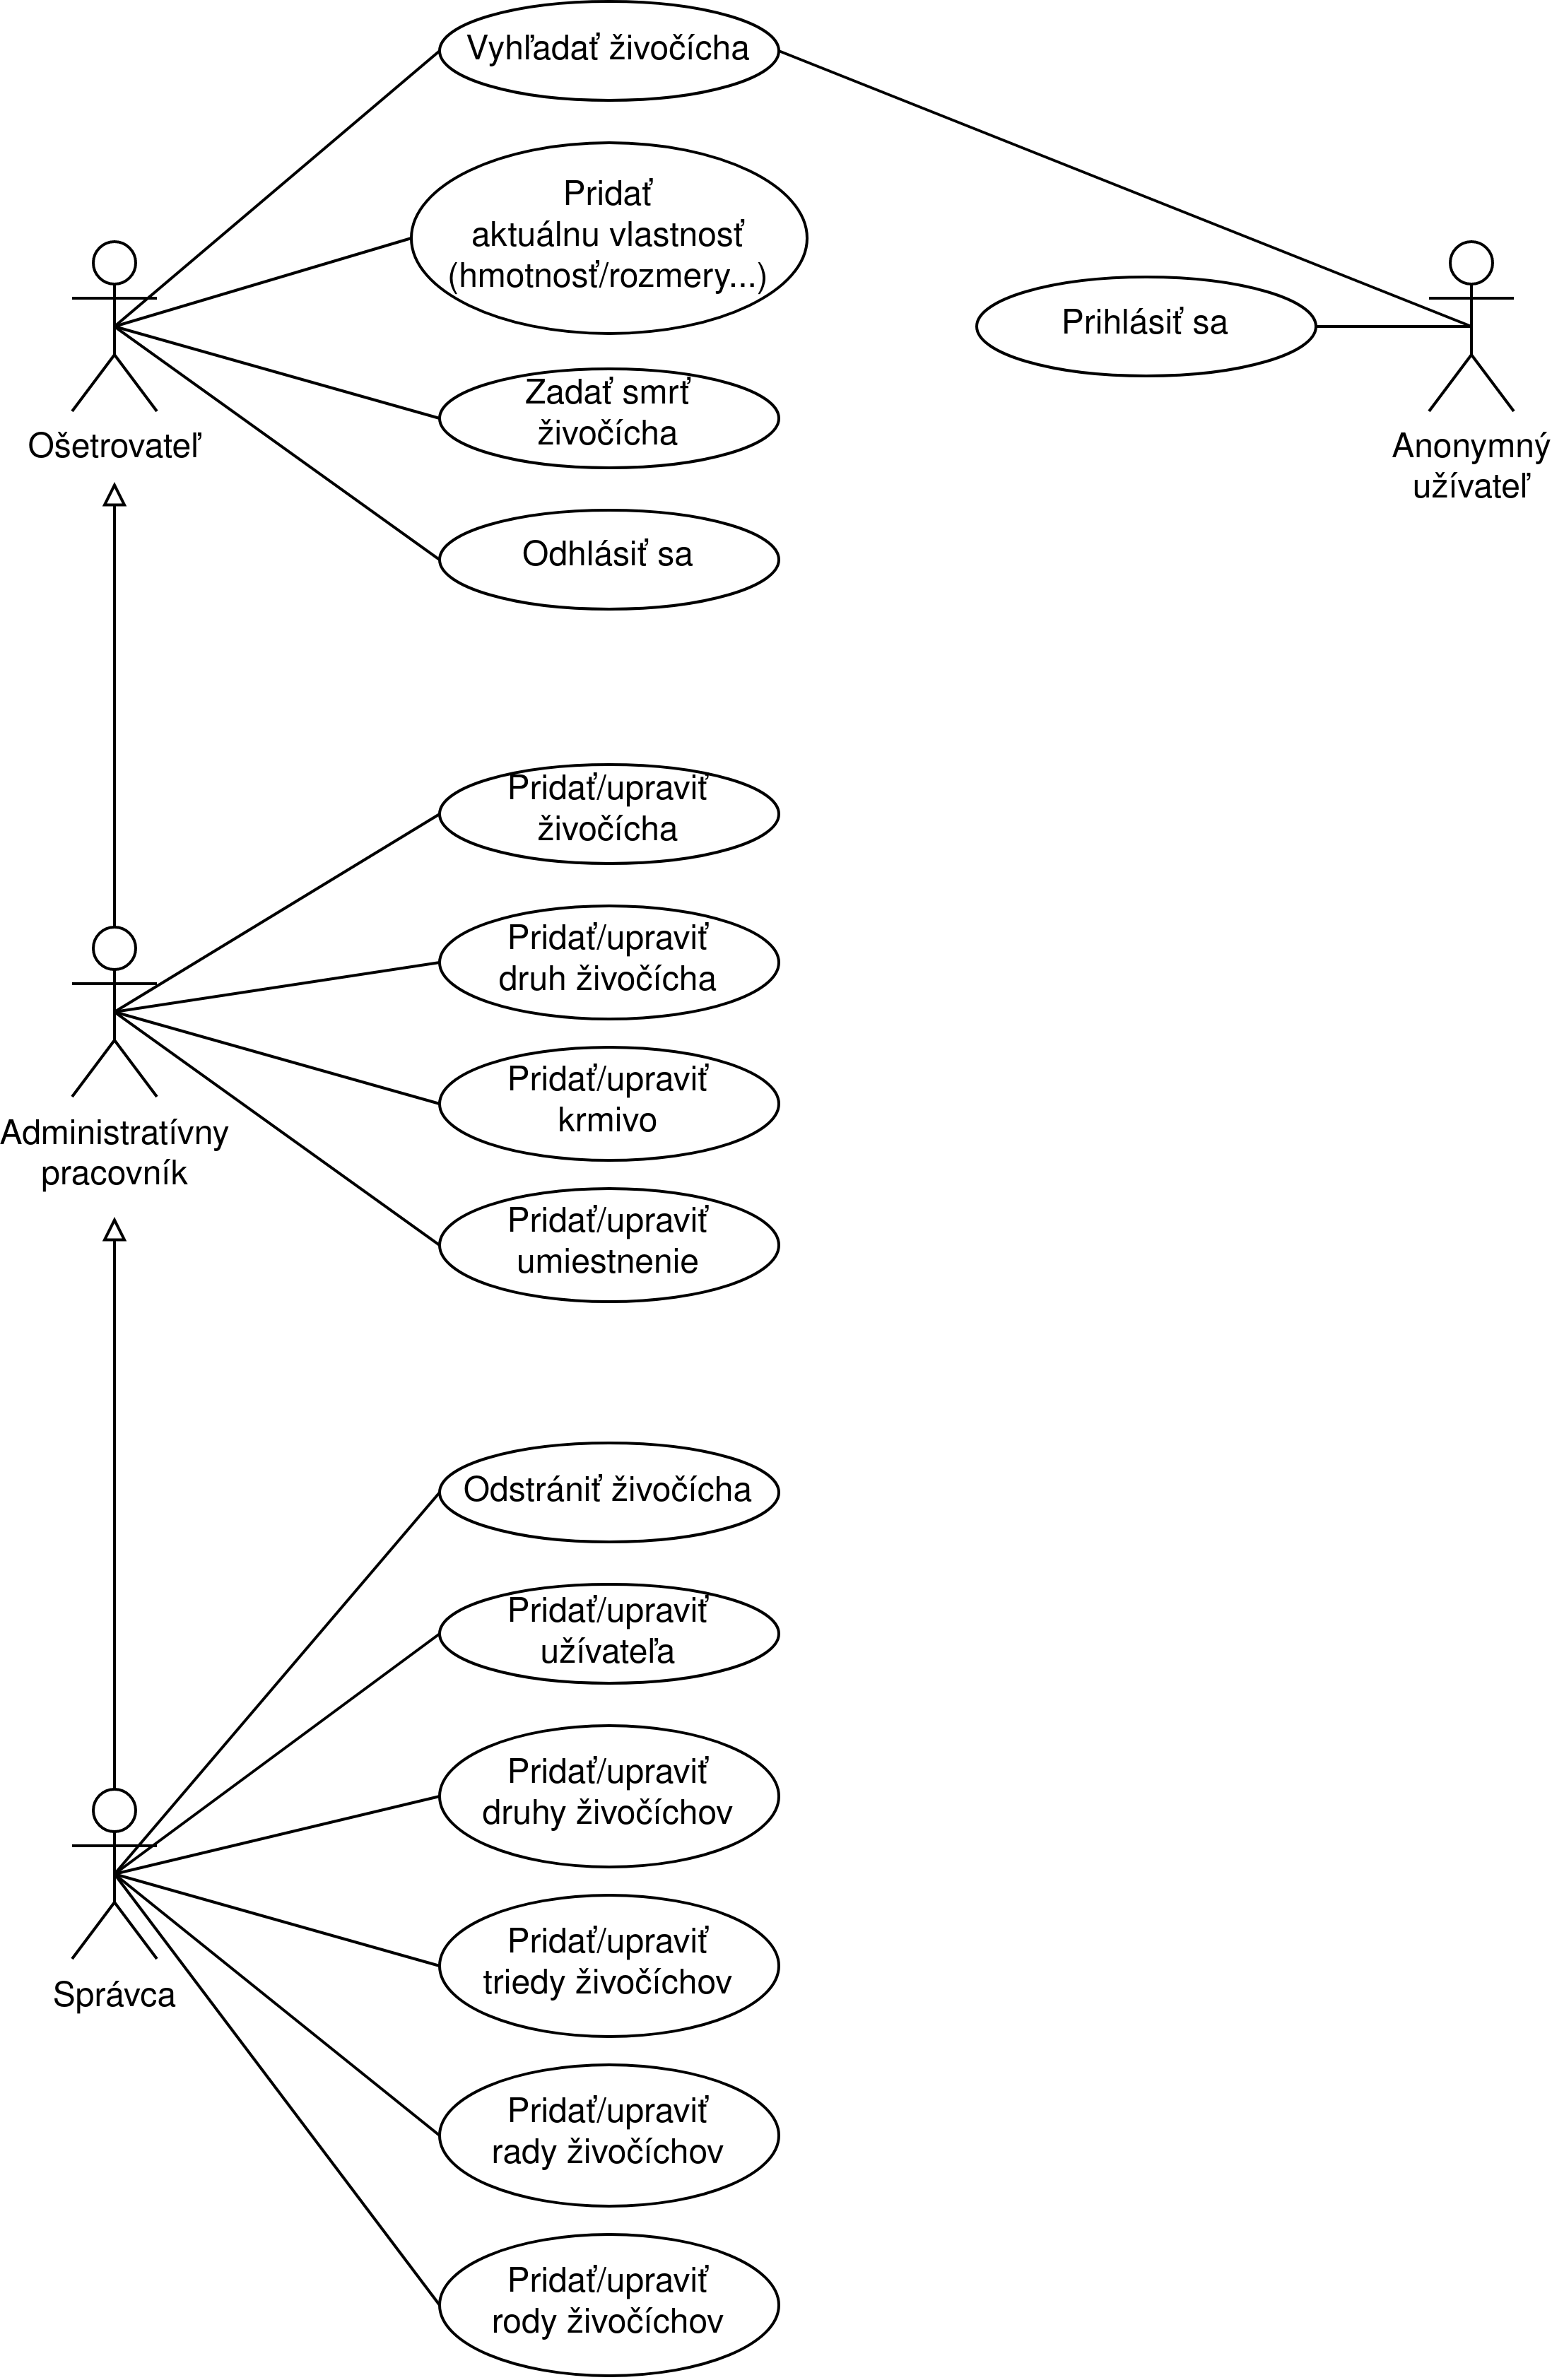
\includegraphics[width=1 \linewidth]{use case.png}}

	        \section{Entity Relationship Diagram}
			\centering
			\scalebox{1.15}{
			\includegraphics[width=0.85 \linewidth]{ER.png}}
\end{document}